%
%  Created by dariogf on 2006-10-19.
%  Copyright (c) 2006 __MyCompanyName__. All rights reserved.
%

\documentclass[12pt,oneside,a4paper,english]{article}  % (fold)

% Use utf-8 encoding for foreign characters
\usepackage[utf8]{inputenc}
%\usepackage[latin1]{inputenc}

\usepackage[english]{babel} %%%Incluimos el paquete Babel que sirve para separar correctamente las palabras de multitud de idiomas%%%

% Setup for fullpage use
\usepackage{fullpage}

\usepackage{indentfirst}
%\usepackage{pdfsync}

\parskip 3ex % distancia entre los párrafos de texto

% Set dimensions of columns, gap between columns, and paragraph indent 
% \setlength{\textheight}{8.875in}
% \setlength{\textwidth}{6.875in}
% \setlength{\columnsep}{0.3125in}
% \setlength{\topmargin}{0in}
% \setlength{\headheight}{0in}
% \setlength{\headsep}{0in}
% \setlength{\parindent}{3em}
% \setlength{\oddsidemargin}{-.1875in}  % Centers text.
% \setlength{\evensidemargin}{-.1875in}

% Uncomment some of the following if you use the features
%
% Running Headers and footers
%\usepackage{fancyheadings}

% Multipart figures
%\usepackage{subfigure}

% More symbols
\usepackage{amsmath}
%\usepackage{amssymb}
%\usepackage{latexsym}

% Surround parts of graphics with box
\usepackage{boxedminipage}

% Package for including code in the document
\usepackage{listings}
\usepackage{xcolor}

\usepackage{colortbl}

% If you want to generate a toc for each chapter (use with book)
\usepackage{minitoc}

% This is now the recommended way for checking for PDFLaTeX:
\usepackage{ifpdf}

%\newif\ifpdf
%\ifx\pdfoutput\undefined
%\pdffalse % we are not running PDFLaTeX
%\else
%\pdfoutput=1 % we are running PDFLaTeX
%\pdftrue
%\fi

\ifpdf
\usepackage[pdftex]{graphicx}
\else
\usepackage{graphicx}
\fi
\graphicspath{{fotos/}}

\bibliographystyle{plain}

\ifpdf
\DeclareGraphicsExtensions{.pdf, .jpg, .tif}
\else
\DeclareGraphicsExtensions{.eps, .jpg}
\fi


 \title{\textbf{AlignMiner v 1.0}\\
		Quick Tutorial}
 
 \author{Darío Guerrero, 
         Rocío Bautista, and 
         M. Gonzalo Claros \\
         Plataforma Andaluza de Bioinformática\\ Universidad de Málaga (Spain)
      }
    
% 
% \date{22-03-2007}

% (end)

\begin{document}
	
%\lstset{language=Java}

\lstset{basicstyle=\scriptsize, commentstyle=\color{blue}}

\maketitle

%\begin{abstract}

%\end{abstract}

%%%%%%%%%%%%%%%%%%%%%%%%%%%%%%%%%%%%%%%%%%%%%%%%%%%%%%%%%%%%%%%%%%%%%
%\section{Introduction}\label{sec:introduction} % (fold)
%%%%%%%%%%%%%%%%%%%%%%%%%%%%%%%%%%%%%%%%%%%%%%%%%%%%%%%%%%%%%%%%%%%%%

{\small This document is only a quick guide to AlignMiner. An in-depth explanation will soon be available when the article that describes it will be published}.

% section introduccion (end)

%\section{Usage}



\subsection*{System login}

First to do in order to use AlignMiner is to allocate your data in the system by a login with your e-mail. Enter any valid email in the form of the main page, as seen in the following picture:

\begin{center}
		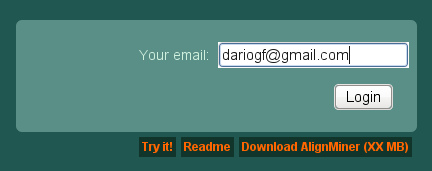
\includegraphics[width=.5\linewidth]{pics/login.jpg}
\end{center}

Once logged in, you can choose between submitting new jobs or browse already sent ones.

\subsection*{Submiting a new job}

Submitting new jobs include uploading a file containing a valid alignment. AlignMiner supports a wide variety of formats (fasta, clustal, msf, ...), so you can try to upload yours without any conversion. Select the alignment to upload using the ``\textbf{Browse...}'' button or write the path in the `\textbf{`File}'' field.

You may also provide a name for the job. If not, an automatically generated number is assigned.

\begin{center}
		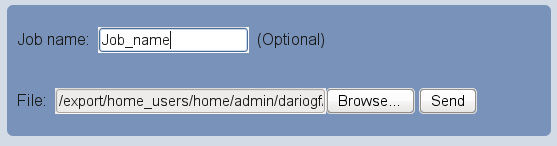
\includegraphics[width=.6\linewidth]{pics/submit.jpg}
\end{center}

Click ``\textbf{Send}'' button to submit the file.

When the file has been successfully uploaded, you will see a new form (and some useful information on the right) where you can select some parameters:

\begin{center}
		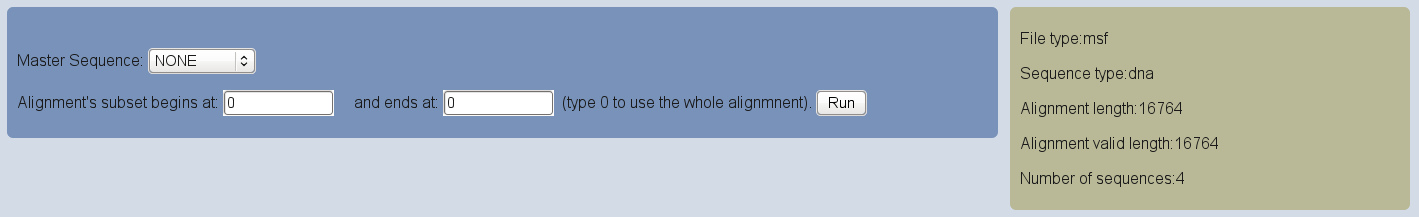
\includegraphics[width=\linewidth]{pics/params.jpg}
\end{center}

\begin{itemize}
\item \textbf{Master sequence}: you can select a master sequence from the popup in order to compare all sequences with respect to the master. If you don't select a master sequence,  a consensus of the whole alignment is then calculated and used as reference.
\item \textbf{Alignment subset}: this enables you to force AlignMiner to analyze only a portion of the alignment. If you leave both fields with zeroes, an automatic range will then be calculated, and weak ends (those with little information) of the alignment will be cropped.
\end{itemize}

Click ``\textbf{Run}'' button to send the job for execution to a batch queue. Your job will appear in the job list

\begin{center}
		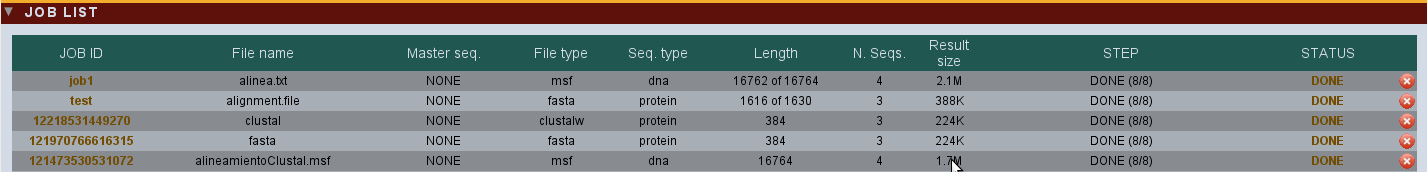
\includegraphics[width=\linewidth]{pics/joblist.jpg}
\end{center}

as well as the execution status:

\begin{center}
		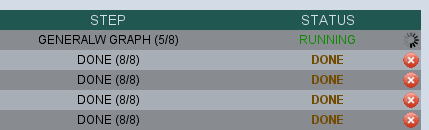
\includegraphics[width=.6\linewidth]{pics/run.jpg}
\end{center}

\begin{itemize}
\item \textsc{Waiting run}: the job has just been uploaded and is waiting for you to click on the ``\textbf{Run}'' button.
\item \textsc{Queued}: the job has been sent to the batch system and is waiting for resources for execution.
\item \textsc{Running}: the job is running. The STEP column is displaying the completed steps.
\item \textsc{Done}: the job is done and available for browsing.
\item \textsc{Error}: there has been an error that prevents the correct execution. You can check the small info icon for more information.
\end{itemize}

You can close the system and come later to see your job status, or wait until finishing.

\subsection*{Browsing previous jobs}

Jobs are saved for further browsing, so you can access the system at any time and choose a job from the job list and browse the results.

If you click on a job name, you get a list of available scoring methods, taking into account that ADNW is only available for nucleic acid alignments, not for protein alignments:

\begin{center}
		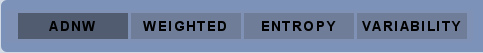
\includegraphics[width=.8\linewidth]{pics/methods.jpg}
\end{center}
		
When a scoring method is selected, a graph is shown for the visual representation of results. You can drag, zoom or click the graph on your own:

\begin{center}
		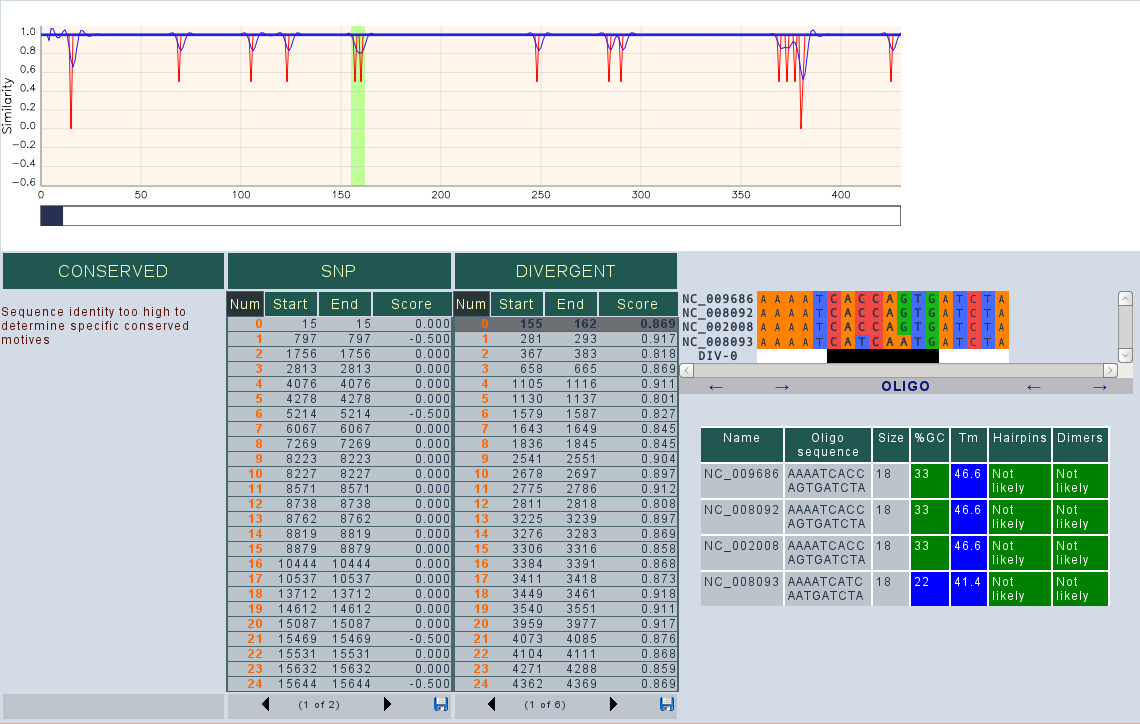
\includegraphics[width=\linewidth]{pics/graph.jpg}
\end{center}

Below the graph, the interesting regions that have been found are presented in tables. You can sort tables by clicking on a column title. When you click on a row (a region of interest), its corresponding alignment is show on the right of the table. In DNA alignments, characteristics of a putative primer based on this region are also calculated. You can change the primer width by clicking on the arrows, and its characteristics will be re-calculated for this new sequence window.

% section futuro (end)

% \nocite{MooneySNP}
% \nocite{SNPEST}
% \nocite{MultipleAlign}
% \nocite{LocalWeighting}
%\nocite{ESTprotocol,SNPEST,MooneySNP,EST2uni,ESTpass,LocalWeighting,preAssemble,autoSNP,SNPServer,MultipleAlign}


%\bibliography{bibliografia}

\end{document}
